% !TeX root = ../report.tex

% Key information to be included:
% - Few lines about the general method and the steps followed
% - Heuristics (report the definitions in the previous slides)
% - Metrics agreed among all evaluators
% - Final scores agreed among all evaluators (include the main comments
% for your scores and examples of commentedscreenshots to support
% your scores)
% - Annex: Report the scores and main comments of EACH evaluator
% - PROVIDE AGGREGATED DATA, e.g., MEAN VALUES FOR ALL EURISTICS,
% (MEAN) SCORE BY DIMENSIONS (e.g., for CONTENT HEURISTICS,
% NAVIGATION HEURISTICS, ect.)
% - PROVIDE VISUAL REPRESENTATIONS OF RESULTS (diagrams, summary
% tables...)
% - Include a short conclusion section where you breifly discuss inspection
% results

\section{Inspection}

\subsection{Method}
% what is inspection based usability evaluation
% specific heuristics and metrics used
\subsubsection{Heuristics}

\subsubsection{Metrics}

\subsection{Execution of the study}
% How the study was performed

\subsection{Results}
% Agreed scores (with comments)
% Aggregates scores (with visualizations)
\paragraph{Nielsen}
    % header
\begin{tabularx}{\linewidth}{l c X}
\toprule
\textbf{Heuristic} & \textbf{Score} & \textbf{Comment} \\
\midrule
\endfirsthead
\toprule
\textbf{Heuristic} & \textbf{Score} & \textbf{Comment} \\
\midrule
\endhead
\midrule
\footnotesize [Continues on next page]
\endfoot
\bottomrule
\endlastfoot
    % body
    H1 & 1 & There is a difficulty in navigation as breadcrumbs are sometimes either missing or incorrect.\par When using the search bar, there is no feedback on the progress status, the page can appear frozen. \\ \midrule
    H2 &  & \\ \midrule
    H3 &  & \\ \midrule
    H4 &  & \\ \midrule
    H5 &  & \\ \midrule
    H6 &  & \\ \midrule
    H7 &  & \\ \midrule
    H8 &  & \\ \midrule
    H9 &  & \\ \midrule
    H10 &  &
\end{tabularx}

\paragraph{Mile}


\begin{tabularx}{\linewidth}{l c c X}
\toprule
\textbf{Category} & \textbf{Heuristic} & \textbf{Score} & \textbf{Comment} \\
\midrule
\endfirsthead
\toprule
\textbf{Category} & \textbf{Heuristic} & \textbf{Score} & \textbf{Comment} \\
\midrule
\endhead
\midrule
\footnotesize [Continues on next page]
\endfoot
\bottomrule
\endlastfoot

\multirow{5}{*}{\textbf{Navigation}}   & MN1 & 0 & Lorem ipsum Lorem ipsum Lorem ipsum Lorem ipsum Lorem ipsum \\ \cmidrule{2-4} 
                                        & MN2 &  &  \\ \cmidrule{2-4} 
                                        & MN3 &  &  \\ \cmidrule{2-4} 
                                        & MN4 &  &  \\ \cmidrule{2-4} 
                                        & MN5 &  &  \\ \midrule
\textbf{Content}                       & MC1 &  &  \\ \midrule
\multirow{5}{*}{\textbf{Presentation}} & MP1 &  &  \\ \cmidrule{2-4} 
                                        & MP2 &  &  \\ \cmidrule{2-4} 
                                        & MP3 &  &  \\ \cmidrule{2-4} 
                                        & MP4 &  &  \\ \cmidrule{2-4} 
                                        & MP5 &  &  \\
\end{tabularx}

\subsection{Discussion of results}
\subsubsection{Discussion within Nielsen's heuristics}
\begin{enumerate}
    \item \textbf{Visibility of system status}\\
    Commento su heuristic (Figura \ref{fig:1-image-ref})
    \begin{figure}[!h]
        \begin{minipage}{\linewidth}
            \centering
            \makebox[\textwidth][c]{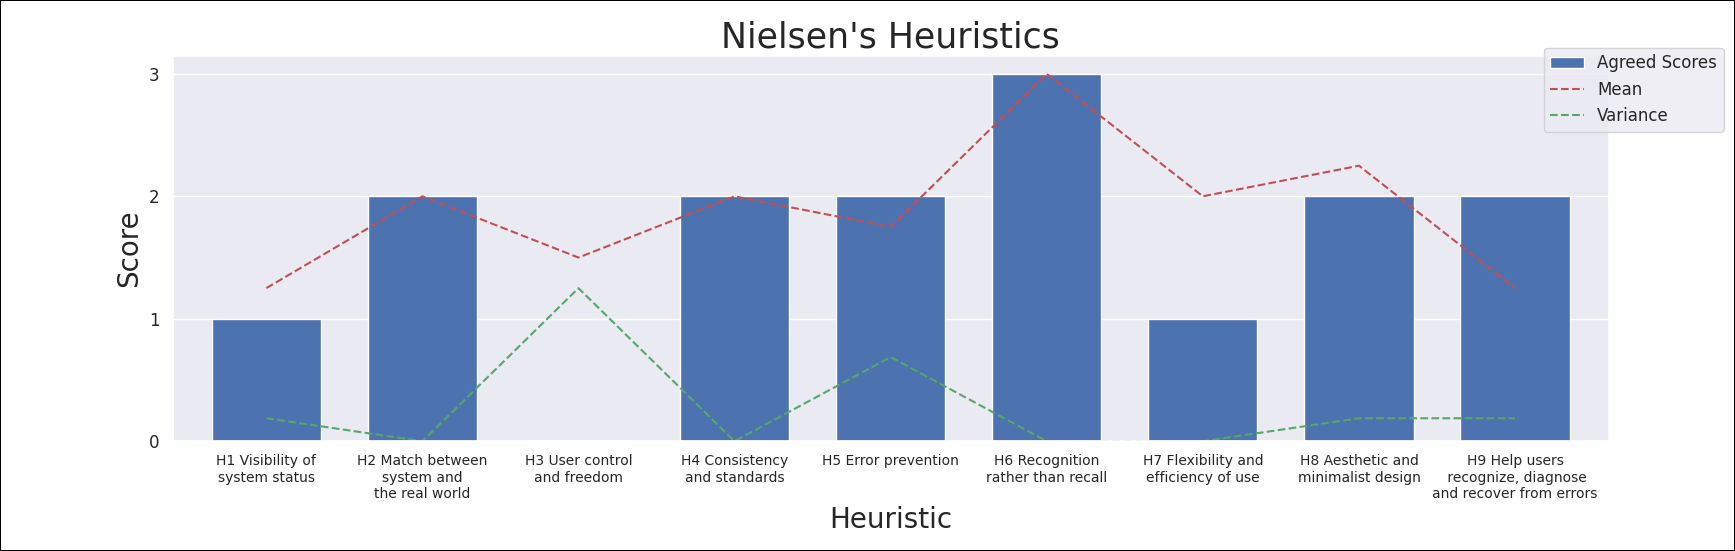
\includegraphics[width=0.8\textwidth]{images/test.png}}%
            \caption{Label dell'immagine}
            \label{fig:1-image-ref}
        \end{minipage}
    \end{figure}
    \item \textbf{Nielsen 2}\\
    Bla bla
    \item bla bla
\end{enumerate}


\subsubsection{Discussion within Mile's heuristics}


\pagebreak
Commento